\section{Neural Networks in Chess}
\label{sec:NeuralNets}

Over the last decade computer engines went from consisting of intelligent efficient search and evaluation algorithms, to being focused on creating larger, and intricate neural network architectures that could reach newer heights when it comes to accuracy and general strength of play. Examples of this include the previously mentioned Stockfish \cite{stockfish2024} and AlphaZero \cite{AlphaZero}. The prior being an amalgamation of using algorithms like MinMax \& Alpha-Beta Pruning (see Section \ref{sec:Chess Programming}) to guide the neural network in finding the most optimal move, while the latter being made up of a neural network that teaches itself the game of chess without prior outside knowledge, using techniques like Monte Carlo Tree Search \cite{Klein}. Both approaches present the different paradigms of creating a strong chess engine, which in turn raises the question "How can one make use of these neural networks to improve how Endgames are played by engines?"

\subsection{Overview}
The main objective of this paper, as highlighted by its title, is to explore how neural networks can be used as a replacement to endgame tablebases in the hope of finding benefits when it comes to the speed of probing, but more importantly to save on the storage space required by the tablebases. For the sake of simplicity and lack of resources, this paper will look into one metric provided by tablebases, and using a neural network in place of the tablebase for probing.

More concretely, the objective is to design a neural network that given a chess position can predict the correct WDL value. Once this is proven feasible, the other metrics can be predicted by the same process. 

\subsection{Pattern Recognition}
\label{subsec:PattRec}
Similar to the process of examining how a Grandmaster would think about the problem of finding the best move in Section \ref{sec:Chess Programming}, using this approach here when given a position and determining the WDL, more abstractly determining whether it is good or bad, can help pinpoint what features make up a position.

In the experiments conducted by de Groot \cite{deGroot} players of varying strength ranging from masters to complete novices were presented with various positions that could arise in a standard game of chess and were given the task of reproducing the position on an empty board after viewing it for a short period of time (3-10 seconds). On average, it was found that master level players were able to more accurately reproduce the position with only a couple of pieces being misplaced, if at all, while novice players showcased having a larger margin of error when recreating the given positions.

On first glance, one could hypothesise that since a master player has spent a long period of time in contact with chess positions that their memory for remembering such positions would be better compared to that of a novice player. Nevertheless, this would be disproven when considering the second set of experiments conducted.

In the second set of experiments both the master and novice player where once again presented with the same task, but this time instead of the positions being those that could come up in a standard game, the players were presented positions where the pieces were placed completely randomly. This time around, the accuracy of the master players significantly dropped in contrast to the first experiment, and was barely better than that of the novice players.

\begin{figure}[H]
    \centering
    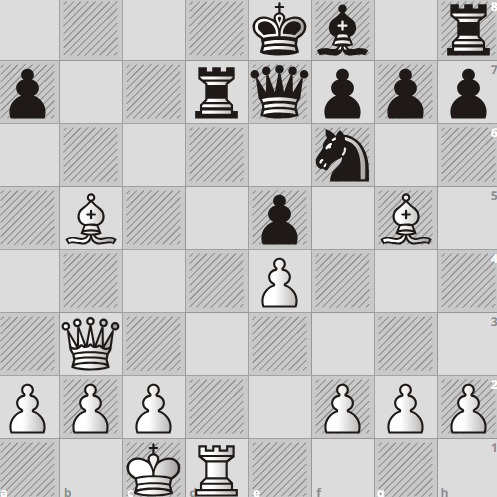
\includegraphics[scale=0.45]{images/MorphyPosition.png}
    \caption{Example of a position that could arise in a game}
    \label{MorphyPosition}
\end{figure}

\begin{figure}[H]
    \centering
    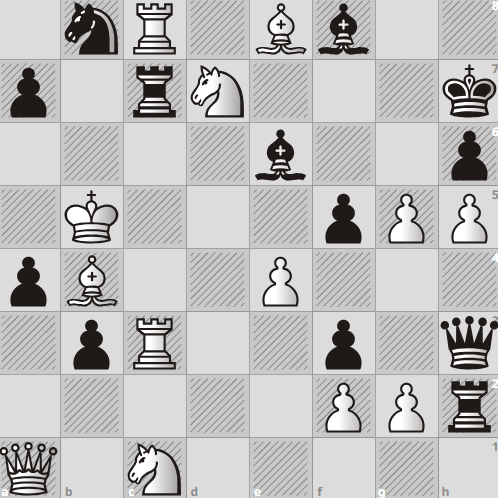
\includegraphics[scale=0.45]{images/RandomPosition.png}
    \caption{Example of a position where the pieces are randomly placed}
    \label{RandomPosition}
\end{figure}

Figures \ref{MorphyPosition} \& \ref{RandomPosition} show visually what a position that could arise from a game, and a random position look like. In Fig.\ref{MorphyPosition} a master player would look at symmetrical pawn structure of white, at the e4 pawn being attacked by the Knight, and the pins (meaning a piece can or should not move when being attacked due to it covering a piece of greater value) placed on the d7 Rook and f6 Knight by the b5 and g5 Bishops respectively. While in Fig.\ref{RandomPosition} the pieces are not \textit{harmonious} with each other and are scattered haphazardly, making it harder to extract the relations and patterns between them. Figure \ref{MorphyAnotated} demonstrates this.

\begin{figure}[H]
    \centering
    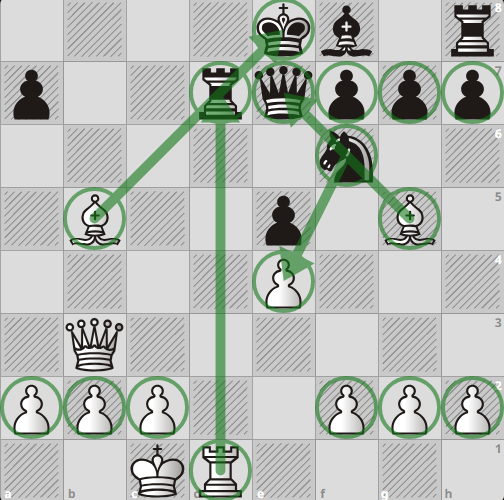
\includegraphics[scale=0.45]{images/MorphyAnotated.png}
    \caption{The patterns a master player would see when observing the position in Fig.\ref{MorphyPosition}}
    \label{MorphyAnotated}
\end{figure}

The process just described is exactly what needs to be done by the neural networks, in order to extract the essential features like pawn structures, relative positions of the pieces to each other, and many more so that it can make an accurate estimation about whether a position is good or not. In simpler words, we need a neural network good at recognising patterns.

\subsection{Convolutional Neural Networks}
Convolutional Neural Network are a special type of neural network architecture used mainly in the field of image/object recognition. When dealing with a grey-scale image like the ones in the MNIST Classification Dataset \cite{MNIST} one could use the traditional Multi-Layer-Perceptron \cite{Klein} where each pixel would have a value ranging from 0 (black) to 255 (white), and the 2x2 grid of pixel would then be converted to a singular 1-dimensional array that is treated as the input of the perceptron, and fully connected to the following hidden layers with the respective weights, biases and activation functions, eventually leading to the output layer containing 10 neurons/nodes each corresponding to a digit 0-9 with the value outputted at each node being the confidence/probability of the given image being the corresponding number represented by the node.
\begin{figure}[H]
    \centering
    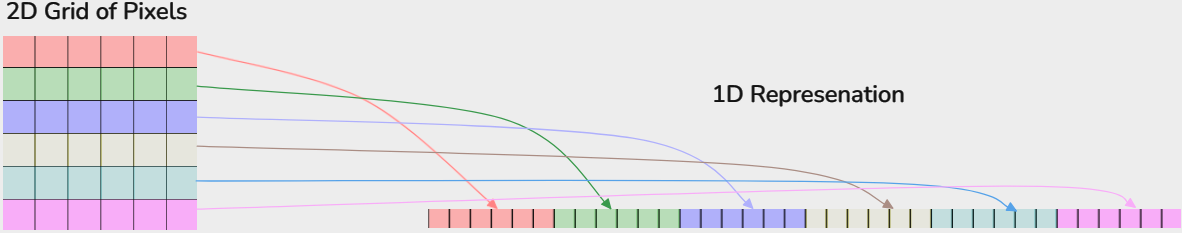
\includegraphics[scale=0.45]{images/2Dto1D.png}
    \caption{Modelling a 2D Grid of Pixels (commonly known as an image) in one dimension}
    \label{2Dto1D}
\end{figure}


With sufficient training data, such a model could be very accurate and reliable in several use cases, but one major problem arises. Scaling. The MNIST Handwritten Digits Dataset contains images of dimension 28x28, in other words there are 784 individual pixels that must each correspond to a single neuron. Furthermore, most images processed in the context of image/object recognition are much larger than the measly 28x28 dimensions of the MNIST Dataset, so in the worst case, one would need to adjust the size of the input layer for each type of image to be processed. This alone increases the complexity of the architecture when using greyscale images, let alone coloured ones.

This is where CNNs shine, their architecture allows for variability in the size of the input images without significantly increasing the size or complexity of the model. The process involves the input going through multiple convolutional layers that contain kernels/filters that pass over the image as a whole and create an output matrix known as a feature map. The size of each convolutional layer depends on the size of the convolutional layer preceeding it and its resepctive kernels. The size of the kernels determines what is known as the receptive field. This tells us how much information from the previous layers is propagated through to the current layer \cite{lecun2015deep}.

\begin{figure}[H]
    \centering
    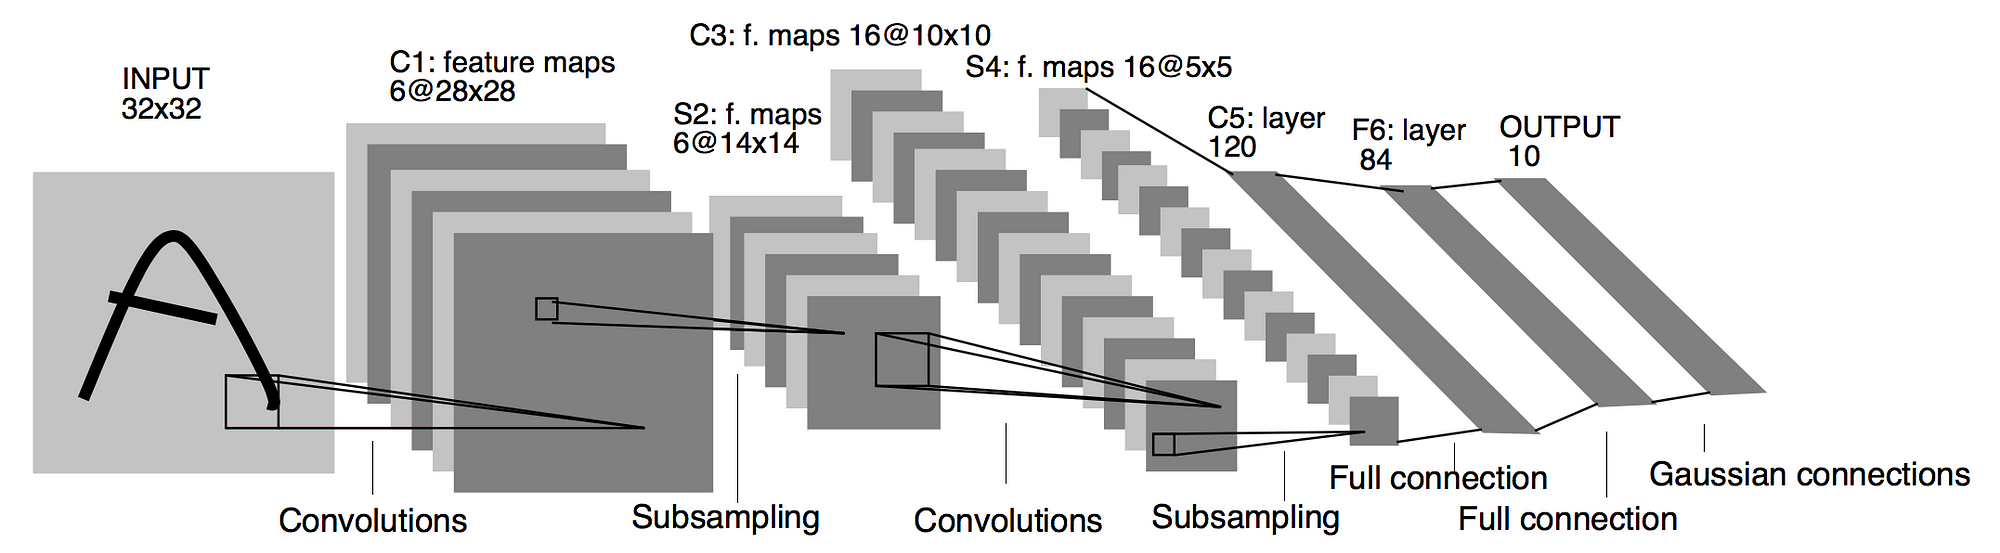
\includegraphics[width=\textwidth]{images/LeNet5Arch.png}
    \caption{Example architecture of LeNet5 \cite{LeNet5} where the kernels and convolutional layers are seen}
    \label{LeNet}
\end{figure}

\subsubsection{Convolution \& Kernels}
Convolution \cite{Goodfellow-et-al-2016} is the fundamental operation that gives CNNs their name and is key to their ability to efficiently process images, or more generally spatial data. In the context of CNNs, convolution is a mathematical operator that involves the input data (such as an image) and the kernel.
The convolution operation slides the kernel over the input data, performing element-wise multiplication at each position and summing the results to produce a single output value. This process is repeated across the entire input, creating a feature map that highlights particular features or patterns in the data.
For a 2D input image I and a kernel K, the convolution operation can be expressed as follows:
\[
(I * K)(i, j) = \sum_{m} \sum_{n} I(i+m, j+n) \cdot K(m, n)
\]
Where $(i,j)$ represents the position in the output feature map, and $(m,n)$ are the coordinates within the kernel.
Let's consider a simple example to illustrate this process:
Suppose we have a 5x5 input image and a 3x3 kernel:

\noindent Input Image:
\[
\begin{bmatrix}
1 & 1 & 1 & 0 & 0 \\
0 & 1 & 1 & 1 & 0 \\
0 & 0 & 1 & 1 & 1 \\
0 & 0 & 1 & 1 & 0 \\
0 & 1 & 1 & 0 & 0 \\
\end{bmatrix}
\]
Kernel:
\[
\begin{bmatrix}
1 & 0 & 1 \\
0 & 1 & 0 \\
1 & 0 & 1 \\
\end{bmatrix}
\]
To compute the first element of the output feature map, we would perform the following calculation:
\[
(1 \cdot 1) + (1 \cdot 0) + (1 \cdot 1) + (0 \cdot 0) + (1 \cdot 1) + (1 \cdot 0) + (0 \cdot 1) + (0 \cdot 0) + (0 \cdot 1) = 4
\]
The kernel then slides over by one position (the stride), and the process is repeated. The final output feature map for this example would be:
\[
\begin{bmatrix}
4 & 3 & 4 \\
2 & 4 & 3 \\
2 & 3 & 4\\
\end{bmatrix}
\]
This example demonstrates how convolution can detect patterns or features. In this case, the kernel is sensitive to diagonal patterns in the input image.
In practice, CNNs use multiple kernels to detect various features, and the convolution operation is typically followed by a non-linear activation function. The kernels' values are learned during the training process, allowing the network to automatically discover important features for the task at hand.

The kernels used within the first several layers are basic like the one used in this example, they can be used for edge detection (whether horizontal or vertical), corner detection, and many other things. Deeper within the architecture of CNNs the kernels begin extracting features that are more abstract and harder to make sense out of, for us as humans.

\subsubsection{Pooling layers \& Padding}
From the example above, one could notice that the convolution of the 5x5 input matrix using a 3x3 kernel, resulted in a feature map output matrix of dimension 3x3. In other words, the essence of the original input matrix (\textit{i.e. image}) was extracted into a smaller matrix. Depending on the situation this extraction into smaller matrices containing the bare minimum when it comes to essential features can be taken further by introducing the concept of pooling \cite{lecun2015deep}.

Briefly, pooling combines features that are similar, in other words in close proximity to one another, and spits out a number that is representative of them. There are 2 types of pooling layers that are commonly used across most CNNs.

\begin{itemize}
    \item Average Pooling Layers
    \item Max Pooling Layers
\end{itemize}

Similar to the use of kernels, in Average Pooling Layers a filter is passed over the elements of the convolved input and the average of these elements is then outputted as a single element of the output matrix. Max Pooling Layers work analogously but take the maximum element instead of an average.

Suppose we have a 4x4 input matrix (which could be the output of a previous convolutional layer):
\[
\begin{bmatrix}
1 & 3 & 1 & 1 \\
2 & 8 & 2 & 0 \\
0 & 4 & 3 & 2 \\
6 & 1 & 0 & 3 \\
\end{bmatrix}
\]
We'll apply both max pooling and average pooling with a 2x2 filter and a stride of 2.

\noindent\textbf{Max Pooling:}
For max pooling, we take the maximum value in each 2x2 region:
\[
\begin{bmatrix}
\max(1,3,2,8) & \max(1,1,2,0) \\
\max(0,4,6,1) & \max(3,2,0,3)\\
\end{bmatrix} =
\begin{bmatrix}
8 & 2 \\
6 & 3 \\
\end{bmatrix}
\]
\textbf{Average Pooling:}
For average pooling, we take the average value in each 2x2 region:
\[
\begin{bmatrix}
\frac{1+3+2+8}{4} & \frac{1+1+2+0}{4} \\
\frac{0+4+6+1}{4} & \frac{3+2+0+3}{4} \\
\end{bmatrix} =
\begin{bmatrix}
3.5 & 1 \\
2.75 & 2 \\
\end{bmatrix}
\]
Both pooling operations reduce the spatial dimensions of the input. Max pooling tends to highlight the strongest features, while average pooling provides a smoother representation of the features.
Padding is another important concept in CNNs. It involves adding extra rows and columns of zeros (or other values) around the input matrix. This is often done to preserve the spatial dimensions after convolution or to ensure that the filter can be applied to border pixels. For example, if we add a padding of 0 to our original 4x4 input, we get:
\[
\begin{bmatrix}
0 & 0 & 0 & 0 & 0 & 0 \\
0 & 1 & 3 & 1 & 1 & 0 \\
0 & 2 & 8 & 2 & 0 & 0 \\
0 & 0 & 4 & 3 & 2 & 0 \\
0 & 6 & 1 & 0 & 3 & 0 \\
0 & 0 & 0 & 0 & 0 & 0 \\
\end{bmatrix}
\]
This padding allows us to apply a 3x3 convolution while maintaining the original 4x4 output dimensions.

\subsubsection{The Classifier}
Following the convolutional and pooling layers, CNNs typically incorporate one or more fully connected (FC) layers, also known as dense layers. These layers serve as the "classifier" part of the network and play a crucial role in interpreting the high-level features extracted by the preceding layers.
In a fully connected layer, each neuron is connected to every neuron in the previous layer, hence the name "fully connected". This structure allows the network to combine global information across the entire feature space, as opposed to the local focus of convolutional layers.
The primary functions of these FC layers include:
\begin{itemize}
\item \textbf{Feature integration:} FC layers combine local features detected by convolutional layers to form a global understanding of the input.
\item \textbf{Non-linear mapping:} When combined with non-linear activation functions, FC layers can model complex, non-linear relationships between features and target outputs.
\item \textbf{Dimensionality reduction:} FC layers often progressively reduce the dimensionality of the data, distilling the most relevant information for the final prediction.
\item \textbf{Task-specific output:} The final FC layer is designed to produce outputs suitable for the specific task at hand, such as classification probabilities or regression values.
\end{itemize}
For instance, in a classification task, the output of the final FC layer typically has neurons corresponding to each possible class. A softmax activation function \cite{Softmax} is often applied to this layer to produce a probability distribution over the classes.
Mathematically, the operation in a fully connected layer can be expressed as:

\[
y = f(Wx + b)
\]

Where $x$ is the input vector, $W$ is the weight matrix, $b$ is the bias vector, $f$ is the activation function, and $y$ is the output vector \cite{Klein}.

It's worth noting that while FC layers provide powerful classification capabilities, they also introduce a large number of parameters to the network. For example, if a convolutional layer outputs a feature map of size 7x7x512, and the first FC layer has 4096 neurons, this single connection would require 7 * 7 * 512 * 4096 = 102,760,448 parameters. This can lead to increased computational requirements and potential overfitting, especially with limited training data \cite{DBLP:journals/corr/abs-1902-02771}.
To mitigate these issues, techniques such as dropout (randomly setting a fraction of inputs to zero during training) are often employed in FC layers. Additionally, some modern architectures have experimented with replacing FC layers with global average pooling, which can drastically reduce the number of parameters while still maintaining good performance.
In the context of transfer learning, the FC layers are often the only parts retrained when adapting a pre-trained CNN to a new task. This allows the network to leverage the general features learned from a large dataset while fine-tuning the final classification for the specific task at hand.

Understanding the role and behavior of fully connected layers is crucial for effectively designing and training CNNs, as they form the bridge between the automated feature extraction of convolutional layers and the final task-specific predictions of the network.

\subsection{Images within Chess}
For the reader, the previous section may seem to have went off on a tangent away from chess and the topic of this paper, but the connection shall be made clear in the paragraphs to follow.

As mentioned in \ref{subsec:PattRec}, the essence of chess mastery lies within recognising patterns, and the previous section outlined how CNNs can be used exactly for that task. It is now only a matter of modelling the problem in a clever way to be able to make use of these CNNs.

\subsubsection{Bitboards}
Consider a black and white image. It can be viewed as grid, modelled as a 2-dimensional array of pixels where each pixel has either a value of 1 (white) or 0 (black). Similarly, a chess position can be modelled in a similar manner. Assume, we have a board containing only white pawns. The board is a grid of squares/fields, modelled as a 2-dimensional array where each square has either a value of 1 (contains a white pawn) or 0 (does not contain a white pawn). This is what bitboards are \cite{BitBoards}. Figure \ref{fig: pawnBitboards} provides a visual example

\begin{figure}[H]
    \centering
    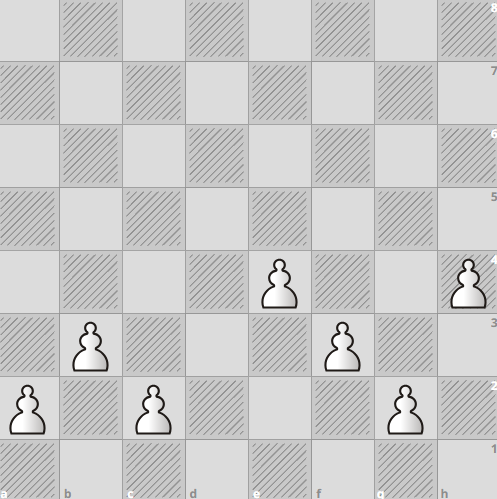
\includegraphics[scale=0.25]{images/PawnBitboard.png}
    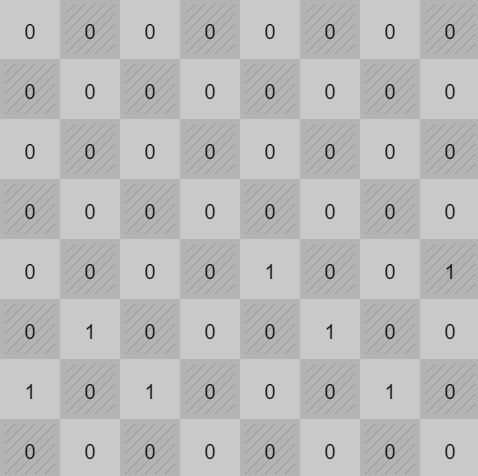
\includegraphics[scale=0.26]{images/PawnBitboardVals.png}
    \caption{Bitboard representation of the white pawns on the board}
    \label{fig: pawnBitboards}
\end{figure}

To represent a colour image, each pixel component (Red, Green, or Blue) is stored on a separate "channel", this allows for dealing with each channel as a single layer in the case of grey-scale images, but instead of 0 being black and 255 being white, 255 would be the colour of the respective channel.

\begin{figure}[H]
    \centering
    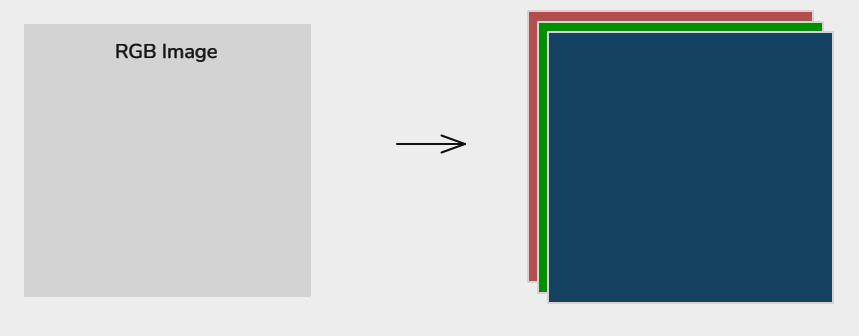
\includegraphics[scale=0.5]{images/RGBtoChannels.png}
    \caption{Decomposition of an RGB Image to Three Channels}
    \label{fig: RGBChannels}
\end{figure}

To represent an entire chess position one would need \textit{at least} 16 bitboards, one for each unique piece (white King, black King, white Queen, black Queen, and so on). Figure \ref{fig: Bitboards} shows a simplified version of this.

\begin{figure}[H]
    \centering
    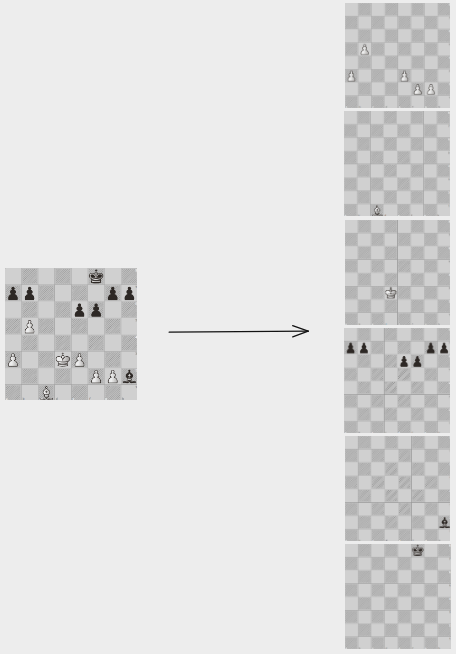
\includegraphics[scale=0.75]{images/BitboardDecomp.png}
    \caption{Decomposition of a position into various bitboards (here as actual pieces for simplicity)}
    \label{fig: Bitboards}
\end{figure}

With that we get a decomposition of what could be a complex chess position into its bare constituents separated over their respective channels, and from that the CNN would be able to come up with its own abstract filter/kernels to make sense and create relations out of the pieces and their positions in order to be able to come up with a concrete value of whether the given position is winning, drawn, or losing for the side to move.

\subsection{Architecture}
\label{Arch}
The CNN architecture chosen is designed to process 12-channel 8x8 input "images". The network consists of three convolutional layers followed by two fully connected layers. The individual layers of the model are visualised in Figure \ref{fig: CNNArch} and are explained below \footnote{It may seem that some kernels are larger than their respective layers, but this is due to the omission of padding in the visualisation}:

\newpage

\begin{itemize}
    \item Input Layer:
    \begin{itemize}
        \item Dimensions: 12 x 8 x 8
        \item The 12 channels each represent the position of a unique type of chess piece on the 8x8 chessboard.
    \end{itemize}
    \item Convolutional Layers:
    \begin{itemize}
        \item Conv1: $12 \rightarrow 64$ channels, 3x3 kernel, padding=1
        \item Conv2: $64 \rightarrow 128$ channels, 3x3 kernel, padding=1
        \item Conv3: $128 \rightarrow 256$ channels, 3x3 kernel, padding=1

        In most modern CNN architectures the number of channels tends to incrementally increase, in order to allow for more complex patterns to be captured and learned so to speak. Additionally, padding is added in order to maintain the spatial dimensions of the "images" and not lose out on the minute details from layer to layer.
    \end{itemize}

    \item Pooling Layers:
    \begin{itemize}
        \item MaxPool2d with 2x2 kernel and stride 2 after each convolutional layer
        
        Pooling reduces spatial dimensions, providing some translation invariance and reducing computational load. The 2x2 pooling halves the spatial dimensions after each convolution, resulting in 4x4, then 2x2, and finally 1x1 feature maps.
    \end{itemize}
    
    \item Flatten Layer
    \begin{itemize}
        \item Converts the 256 x 1 x 1 Tensor to a 256 dimension vector.
    \end{itemize}
    
    \item Fully Connected Layers:
    \begin{itemize}
        \item FC1: $256 \rightarrow 512$ neurons
        \item FC2: $512 \rightarrow 5$ neurons (output layer)
        
        The first FC layer expands the representation to allow for more complex combinations of the learned features. The final layer reduces to 5 outputs, corresponding to the 5 possible values of the WDL metric. This part of the model is where the classification occurs.
    \end{itemize}
    
    \item Activation Functions:
    \begin{itemize}
        \item ReLU after each convolutional and the first fully connected layer
        
        ReLU introduces non-linearity without suffering from vanishing gradient problems \cite{krizhevskyAlexNet}, allowing for effective training of deep networks.
    \end{itemize}
\end{itemize}

\begin{figure}[H]
    \centering
    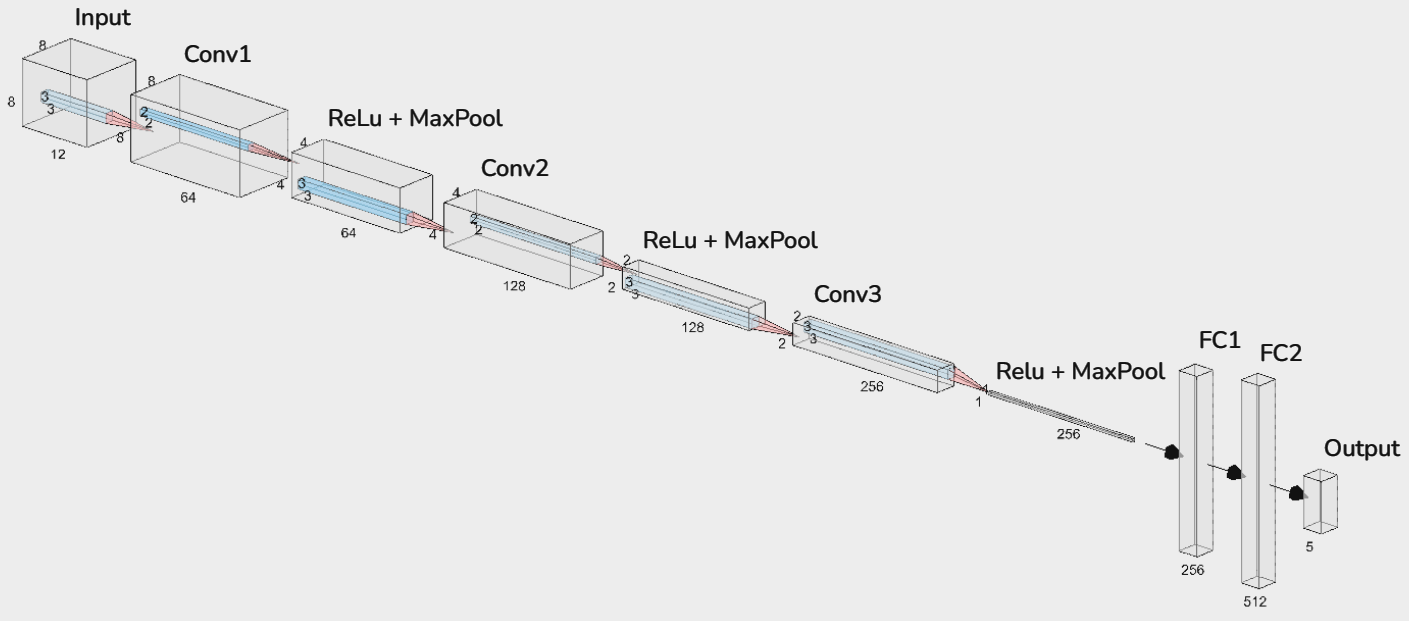
\includegraphics[width = \textwidth]{images/CNNArchitectureLabelled.png}
    \caption{Endgame CNN Model Architecture}
    \label{fig: CNNArch}
\end{figure}

This architecture progressively reduces spatial dimensions while increasing the number of features, a common pattern in CNNs. The choice of layer sizes balances the need for feature extraction (through increasing channel counts) with the constraints of the input size. Starting with 64 channels and doubling to 128, then doubling again to 256, allows for a rich feature hierarchy without excessive computational demands given the small 8x8 input size. The use of powers of 2 for the layer sizes is also another common approach that makes use of the efficient computation of GPUs which usually have operations optimised on power of 2 sized arrays, while also keeping the process of memory access due to the used addressing schemes.

The modern CNN architectures chosen as inspiration for the Endgame Model are mainly AlexNet \cite{krizhevskyAlexNet} and ResNet \cite{heResNet}, due to them establishing significant breakthroughs in the context of image classification \cite{ImageNet}

\subsection{Training}
With the model architecture now in place, the next step is to train it to achieve the desired outcome. The training step can be simplified into the following:

\begin{enumerate}
    \item Create a dataset consisting of the features that are relevant to the prediction, and the expected output value for these respective features.
    \item Split the dataset into training and testing data
    \item Allow the model to iterate through the training data, and adjust its internal randomly initialised weights accordingly
    \item Test the chosen weights using the testing data, and compare it to the actual expected output
    \item Repeat from the second step until a satisfactory accuracy is reached
\end{enumerate}

\subsubsection{Dataset}
To create the dataset needed for training one must first thing about how the functionality of the model would be used. In our case, we want to replace tablebases. Tablebases are provided with a position and are probed in order to output the specific metric we're after (in this case WDL). This would mean our dataset should consist of a representation of a chess position as the \textit{feature} and the WDL as the \textit{target}. In other words all we need are two list containing the features, and their respective targets.

There are several options to acquiring chess endgame positions. Several collections of millions upon millions of games are publicly available online, some of them containing only games of the highest rated players \cite{liDB}\cite{liEliteDB}. These are valid ways of acquiring endgame position, the drawback to them would be that one would need to parse all the games so that only 6-man positions are considered.

The method chosen in this paper was to write a script capable of generating all FENs of positions containing 6 pieces or fewer \cite{FEN}, with that the need for precomputing the games is removed, since the endgame position is directly created. Due to the nature of neural networks and how they \textit{learn} the data in order to find the ideal weights/kernel sizes for each layer, the larger that the dataset used is the higher the chances of improving the model's accuracy are, therefore the dataset used contains 1,000,000 endgame positions alongside their correct WDL evaluation.

\subsubsection{Training Loop}
The training loop is the core process where the model learns from the data \cite{TrainingPyTorch}. It involves repeatedly exposing the model to the training data, computing the loss, and adjusting the model's parameters to minimize this loss. It works as follows:

\begin{enumerate}
    \item Batch Processing: The training data is divided into batches. This allows for more efficient computation and helps in generalising the model by introducing some noise in the gradient computations.
    \item Forward Pass: For each batch, the model performs a forward pass. The input data (12x8x8 Bitboard representation of FEN) is fed through the network, resulting in predictions for the desired outcome (WDL).
    \item Loss Computation: The model's predictions are compared to the actual WDL values using a loss function. In this case, we use the cross-entropy loss function \cite{mao2023crossentropylossfunctionstheoretical}, which is particularly suitable for multi-class classification problems like our WDL prediction.
    \item Backpropagation: The gradients of the loss with respect to the model's parameters are computed using backpropagation. This process calculates how much each parameter contributed to the error.
    \item Parameter Update: The model's parameters are updated using an optimization algorithm (e.g., Stochastic Gradient Descent or Adam \cite{Goodfellow-et-al-2016}) to minimize the loss.
    \item Iteration: Steps 2-5 are repeated for each batch in the training data, constituting one epoch. Multiple epochs are typically performed to refine the model's performance.
    
\end{enumerate}

\paragraph{Cross-Entropy Loss Function}
The cross-entropy loss function \cite{crossentropyloss} is used in this model due to its effectiveness in multi-class classification tasks. It measures the dissimilarity between the predicted probability distribution and the actual distribution of the WDL outcomes.
For a single training example, the cross-entropy loss is defined as:
\[
L = -\sum_{i=1}^{C} y_i \log(\hat{y}_i)
\]
Where:
\begin{itemize}
\item $C$ is the number of classes (in our case, 3 for Win, Draw, Loss)
\item $y_i$ is the true probability of class $i$ (either 0 or 1 in our one-hot encoded targets)
\item $\hat{y}_i$ is the predicted probability of class $i$
\end{itemize}
The loss is minimized when the predicted probabilities closely match the true probabilities. In our case, since each position has only one correct WDL value, the true probability will be 1 for the correct class and 0 for the others.
The use of cross-entropy loss encourages the model to be confident in its correct predictions while heavily penalizing confident incorrect predictions. This aligns well with our goal of accurately classifying chess endgame positions into Win, Draw, or Loss categories.
During training, the model aims to minimize this loss function across all training examples, effectively learning to accurately predict the WDL values for given chess positions.

\subsection{Results}
Two versions of the model were trained, one using 10 Epochs (a.k.a. iterations of the training loop) and the other trained using 50. The relevant metrics throughout the epochs are the training and validation loss (calculated with the previously mentioned Cross Entropy Loss).

The following Plots visualise how these change, alongside a Plot of the accuracy of each model.

\begin{figure}[H]
    \centering
    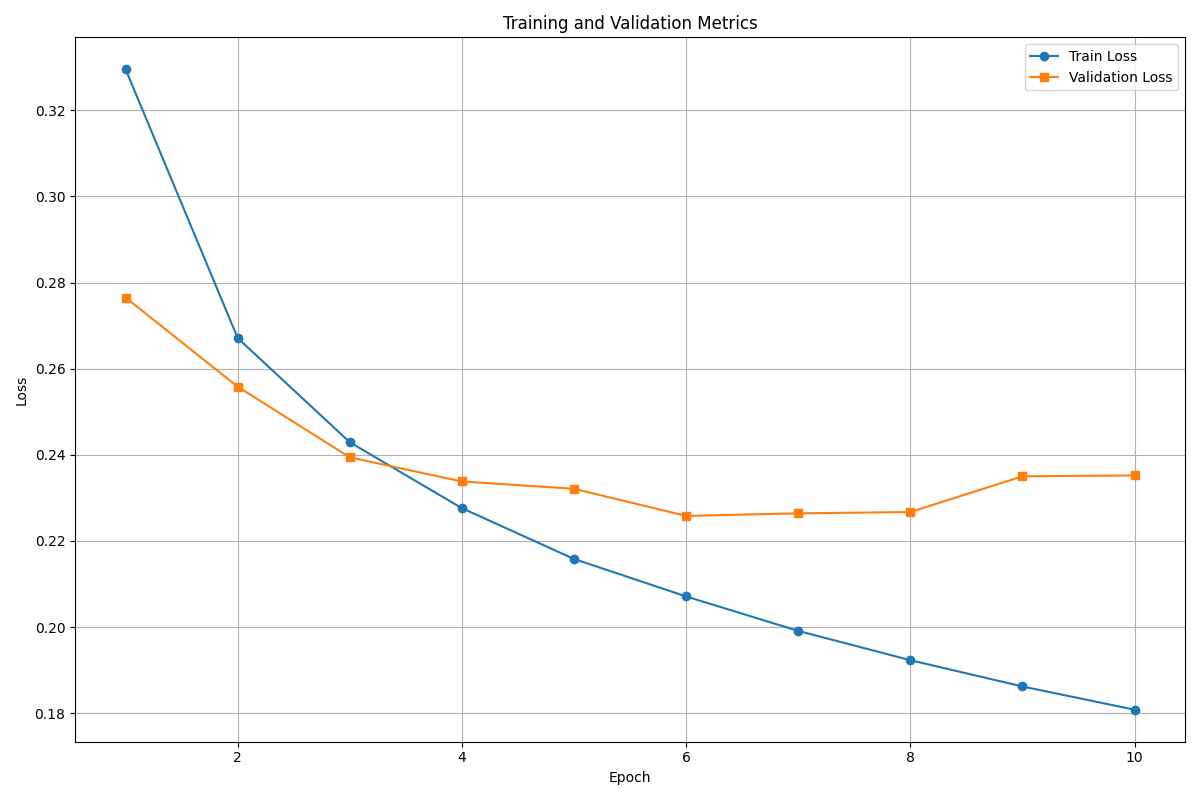
\includegraphics[scale=0.35]{images/10EpochTrainValLoss.png}
    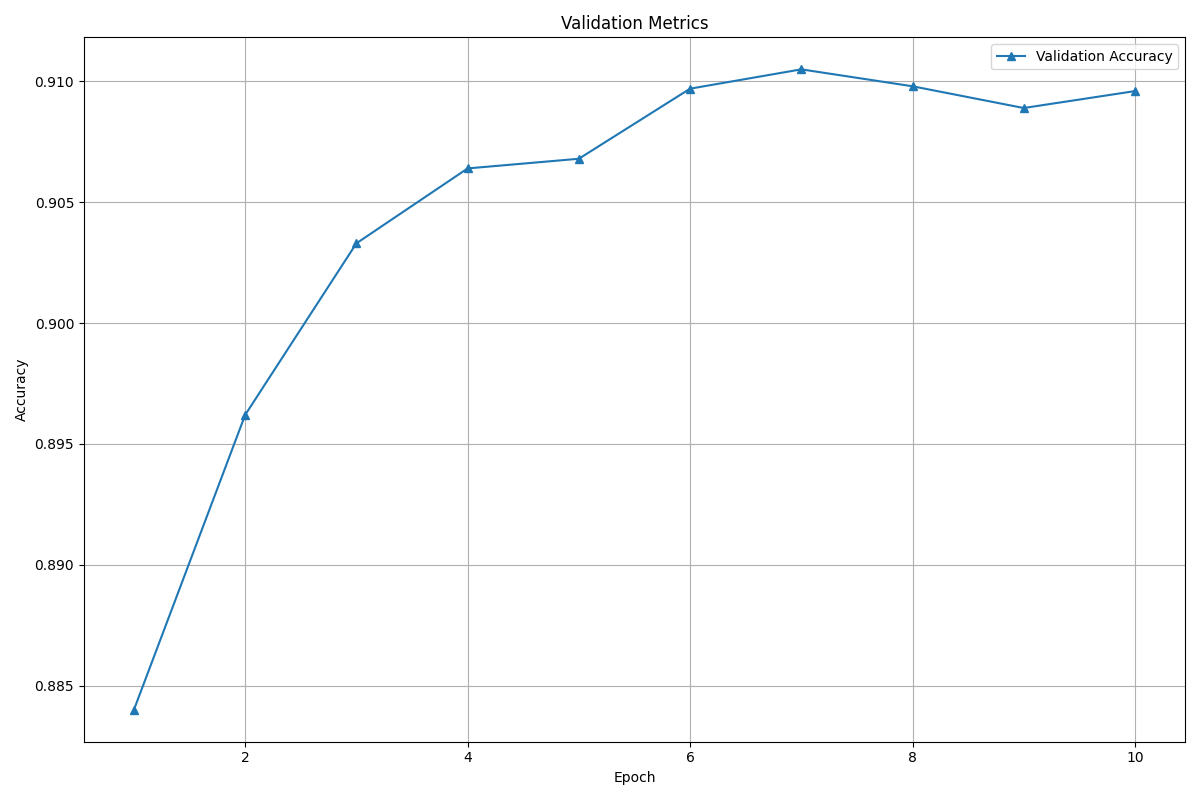
\includegraphics[scale=0.35]{images/10EpochValAcc.png}
    \caption{Training and Validation Loss alongside Validation Accuracy for 10 Epochs}
    \label{fig: 10epoch Metrics}
\end{figure}

\begin{figure}[H]
    \centering
    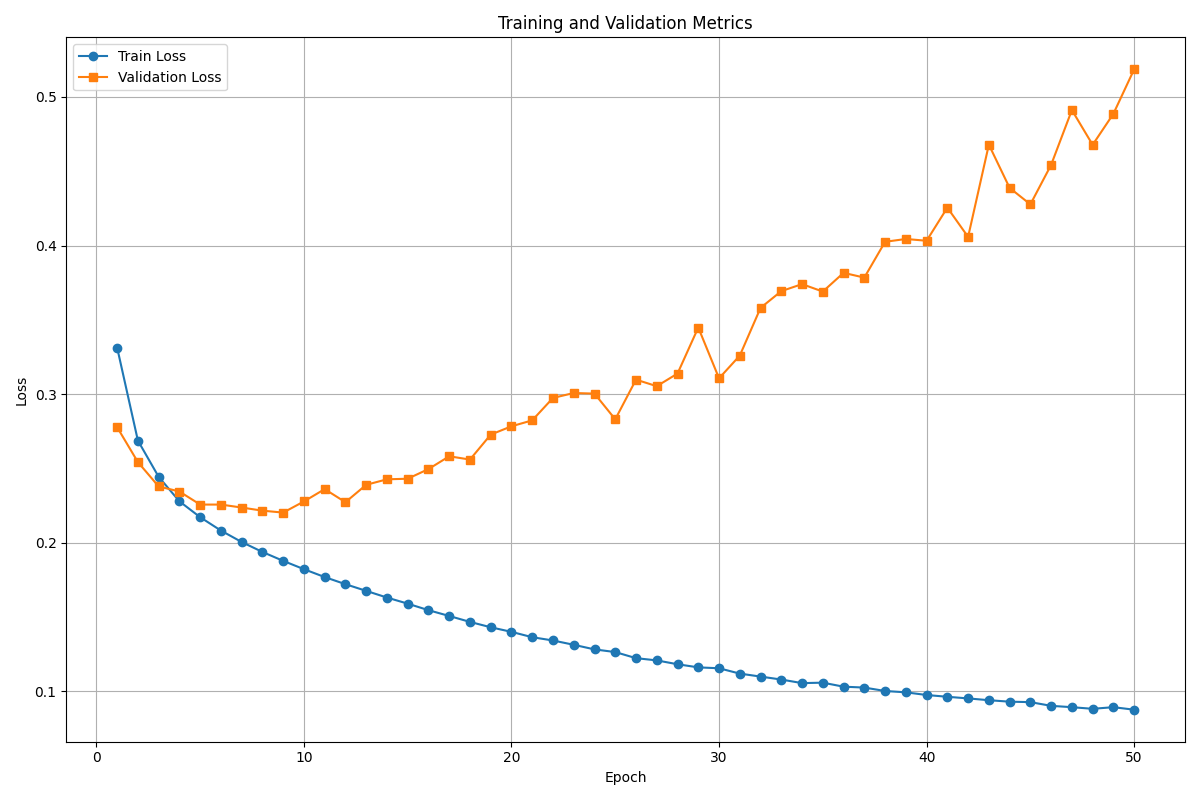
\includegraphics[scale=0.35]{images/50EpochTrainValLoss.png}
    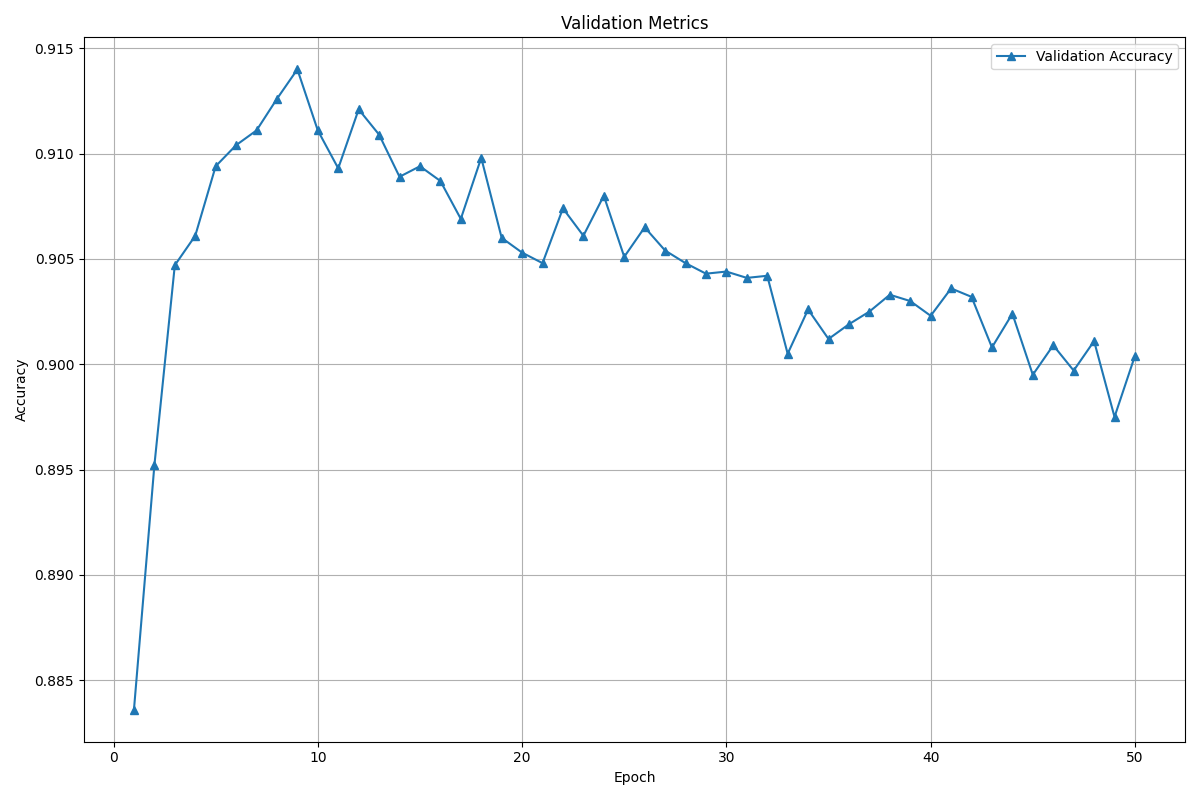
\includegraphics[scale=0.35]{images/50EpochValAcc.png}
    \caption{Training and Validation Loss alongside Validation Accuracy 50 Epochs}
    \label{fig: 50epoch Metrics}
\end{figure}

We notice that after 10 epochs the model begins to have an increasing validation loss, this usually points towards the fact that the model is overfitting. This essentially means that instead of learning patterns, and generalising these findings accross the possible positions it could face, the model starts to memorise the specific inputs it gets. This in turn leads to a decrease in the accuracy of the predicted values.

A possible reason for this happening, would be the "limited" sample space. The amount of patterns that the model could learn isn't that large when there are at most 6 figures on the board. This would lead to the model coming across similar or even identical patterns several times as it goes through the training dataset. This repeated exposure to the same pattern leads to the model simply memorising the output that is expected whenever it faces that said pattern.
\newpage
When it comes to practical use below is an example of the models being used to probe a position.

\begin{lstlisting}[caption= Example comparing output of both models to Syzygy 6-man Tablebase]
Input FEN: 8/K2p4/8/8/6P1/3P4/Q7/2k5 w - - 0 1
. . . . . . . .
K . . p . . . .
. . . . . . . .
. . . . . . . .
. . . . . . P .
. . . P . . . .
Q . . . . . . .
. . k . . . . .
Predicted WDL (50 Epoch Model): 2 (0.172 s)
Predicted WDL (10 Epoch Model): 2 (0.016 s)
Actual WDL: 2 (0.093 s)
\end{lstlisting}

On average the standard approach of probing the tablebase, and loading the 10 epoch model and predicting the WDL for the input FEN have very close times. The main difference would be to the 50 Epoch model.

Below is a practical comparison of the models with 1000 randomly generated FEN strings.

\begin{lstlisting}[caption=Practical comparision of accuracy between models]
No. of tested FENs: 1000
10 Epoch Accuracy: 0.921
50 Epoch Accuracy: 0.910
\end{lstlisting}

This comparison only takes into consideration the time needed to load the weights of the trained models and using them to predict the WDL of the given position.

The actual training time was left out in this section due to it varying depending on the hardware on which it was trained. The hardware used in this case was the NVIDIA GeForce GTX 1650 GPU which is considered to be on the lower end of the today's GPU, but with the help of CUDA \cite{Cuda} it was possible to vectorise the process of training the model by using PyTorch Tensors \cite{PyTorchtensors}, allowing the complete utilisation of the GPU. With that in mind, the training of both models took an accumulative time of around 3 hours.

Having the models predict the WDL in a somewhat comparable time frame to the tablebase probing it is a nice advantage but the main objective here was to significantly decrease the amount of storage space required.

The storage would mostly be needed for the dataset used to train the models, and once that step is done, we'll need to store the weights of the trained models. With the help of the NumPy library, alongside using PyTorch to extract and store the weights in a convenient compatible way lead to them needing no more than 3-5GBs of storage all together.

This is a substantial decrease in the storage needs compared to the nearly 70GBs of storage needed just for the WDL Tablebase. The drawback is that the prediction are no longer perfect, but with a more carefully tailored dataset, or cleverly optimised CNN Architecture the accuracy could be increased even more.

\subsection{Shortcomings}
Some readers may have noticed what could only seem like a logical fallacy when the dataset and its creation were first mentioned. The tablebase was used to create the dataset for the model trained to replace said tablebase. In other words, we use the tablebase to replace the tablebase.

As foolish as it may sound at first, this has its reason. The original aspect of this paper was to take a zero-knowledge base approach. This means that the neural network would learn to evaluate positions from randomly guessing WDL values at first, and with the help of a function that rewards the model when it guesses correctly and penalises it heavily when its wrong, to accurately returning the desired output value. In essence, it would be a process of trial and error.

This approach is how Alpha-Zero \cite{AlphaZero} was capable of training itself towards chess mastery in less than a day.

As it was mentioned in Klein's Chapter of implementing AlphaZero techniques in HexaPawnZero \cite{Klein}, programming a zero-knowledge base neural networks requires colossal amounts of computing power that simply were not readily available in the volume necessary to make this possible, and could theoretically last many hours longer training.

Assuming one could gain access to sufficient computing power, this would be an interesting continuation of this paper, perhaps on tablebases with 3-5 pieces as a start.

Another major point of improvement would be the design of the CNN architecture. The architecture proposed in Section \ref{Arch} was settled upon by a series of trial and error experiments comparing the different outcomes, while also using the pointers mentioned in Stanford's CS231n course as a guide \cite{cs231n}. I was attempting to find a good balance between the resulting models and their accuracies, alongside ensuring that the training time does not take excessively long.

The training time could also be a limiting factor if not dealt with properly. There were several points throughout the process that took several hours to deal with. For instance, downloading the tablebase metrics was no easy task, but even after writing my own script \cite{NeuralBases} to download them, it took a little over an hour to have all the necessary files available locally. When it comes to training the models, the 10 Epoch model took on average 40 minutes to complete its training, while the 50 Epoch model took around 90 minutes.

The different versions of the concrete implementations, could be found in my code repository titled \textit{"NeuralBases"} \cite{NeuralBases}. It showcases how the end goal was incrementally refined. Initially, the idea was to create a chess playing neural network and compare it to the use of the tablebase in assisting a minimal implementation of a MinMax Chess engine. Upon closer inspection, this idea was scrapped due to it not being a fair comparison.

The objective of a tablebase is to provide metrics about the given positions. Therefore, the original idea would be limited by how good my own implementation of the chess engine is, and would give an inaccurate representation of the true capabilities of tablebases. At the end, I settled on comparing the ability of neural networks to come up with the same metrics (in this case only the WDL) as those of the tablebase.

